\documentclass{beamer}

\pdfmapfile{+sansmathaccent.map}


\mode<presentation>
{
	\usetheme{Warsaw} % or try Darmstadt, Madrid, Warsaw, Rochester, CambridgeUS, ...
	\usecolortheme{seahorse} % or try seahorse, beaver, crane, wolverine, ...
	\usefonttheme{serif}  % or try serif, structurebold, ...
	\setbeamertemplate{navigation symbols}{}
	\setbeamertemplate{caption}[numbered]
} 


%%%%%%%%%%%%%%%%%%%%%%%%%%%%
% itemize settings


%%%%%%%%%%%%%%%%%%%%%%%%%%%%
% itemize settings

\definecolor{myhotpink}{RGB}{255, 80, 200}
\definecolor{mywarmpink}{RGB}{255, 60, 160}
\definecolor{mylightpink}{RGB}{255, 80, 200}
\definecolor{mypink}{RGB}{255, 30, 80}
\definecolor{mydarkpink}{RGB}{155, 25, 60}

\definecolor{mypaleblue}{RGB}{240, 240, 255}
\definecolor{mylightblue}{RGB}{120, 150, 255}
\definecolor{myblue}{RGB}{90, 90, 255}
\definecolor{mygblue}{RGB}{70, 110, 240}
\definecolor{mydarkblue}{RGB}{0, 0, 180}
\definecolor{myblackblue}{RGB}{40, 40, 120}

\definecolor{mygreen}{RGB}{0, 200, 0}
\definecolor{mygreen2}{RGB}{245, 255, 230}

\definecolor{mygray}{gray}{0.8}
\definecolor{mydarkgray}{RGB}{80, 80, 160}

\definecolor{mydarkred}{RGB}{160, 30, 30}
\definecolor{mylightred}{RGB}{255, 150, 150}
\definecolor{myred}{RGB}{200, 110, 110}
\definecolor{myblackred}{RGB}{120, 40, 40}

\definecolor{mygreen}{RGB}{0, 200, 0}
\definecolor{mygreen2}{RGB}{205, 255, 200}

\definecolor{mydarkcolor}{RGB}{60, 25, 155}
\definecolor{mylightcolor}{RGB}{130, 180, 250}

\setbeamertemplate{itemize items}[default]

\setbeamertemplate{itemize item}{\color{myblackblue}$\blacksquare$}
\setbeamertemplate{itemize subitem}{\color{mygblue}$\blacktriangleright$}
\setbeamertemplate{itemize subsubitem}{\color{mygray}$\blacksquare$}

\setbeamercolor{palette quaternary}{fg=white,bg=mydarkgray}
\setbeamercolor{titlelike}{parent=palette quaternary}

\setbeamercolor{palette quaternary2}{fg=black,bg=mypaleblue}
\setbeamercolor{frametitle}{parent=palette quaternary2}

\setbeamerfont{frametitle}{size=\Large,series=\scshape}
\setbeamerfont{framesubtitle}{size=\normalsize,series=\upshape}





%%%%%%%%%%%%%%%%%%%%%%%%%%%%
% block settings

\setbeamercolor{block title}{bg=red!30,fg=black}

\setbeamercolor*{block title example}{bg=mygreen!40!white,fg=black}

\setbeamercolor*{block body example}{fg= black, bg= mygreen2}


%%%%%%%%%%%%%%%%%%%%%%%%%%%%
% URL settings
\hypersetup{
	colorlinks=true,
	linkcolor=blue,
	filecolor=blue,      
	urlcolor=blue,
}

%%%%%%%%%%%%%%%%%%%%%%%%%%

\renewcommand{\familydefault}{\rmdefault}

\usepackage{amsmath}
\usepackage{mathtools}

\usepackage{subcaption}

\usepackage{qrcode}

\DeclareMathOperator*{\argmin}{arg\,min}
\newcommand{\bo}[1] {\mathbf{#1}}

\newcommand{\R}{\mathbb{R}} 
\newcommand{\T}{^\top}     

\newcommand{\dx}[1] {\dot{\mathbf{#1}}}
\newcommand{\ma}[4] {\begin{bmatrix}
		#1 & #2 \\ #3 & #4
\end{bmatrix}}
\newcommand{\myvec}[2] {\begin{bmatrix}
		#1 \\ #2
\end{bmatrix}}
\newcommand{\myvecT}[2] {\begin{bmatrix}
		#1 & #2
\end{bmatrix}}


\newcommand{\mydate}{Spring 2023}

\newcommand{\mygit}{\textcolor{blue}{\href{https://github.com/SergeiSa/Control-Theory-Slides-Spring-2023}{github.com/SergeiSa/Control-Theory-Slides-Spring-2023}}}

\newcommand{\myqr}{ \textcolor{black}{\qrcode[height=1.5in]{https://github.com/SergeiSa/Control-Theory-Slides-Spring-2023}}
}

\newcommand{\myqrframe}{
	\begin{frame}
		\centerline{Lecture slides are available via Github, links are on Moodle}
		\bigskip
		\centerline{You can help improve these slides at:}
		\centerline{\mygit}
		\bigskip
		\myqr
	\end{frame}
}


\newcommand{\bref}[2] {\textcolor{blue}{\href{#1}{#2}}}

%%%%%%%%%%%%%%%%%%%%%%%%%%%%
% code settings

\usepackage{listings}
\usepackage{color}
% \definecolor{mygreen}{rgb}{0,0.6,0}
% \definecolor{mygray}{rgb}{0.5,0.5,0.5}
\definecolor{mymauve}{rgb}{0.58,0,0.82}
\lstset{ 
	backgroundcolor=\color{white},   % choose the background color; you must add \usepackage{color} or \usepackage{xcolor}; should come as last argument
	basicstyle=\footnotesize,        % the size of the fonts that are used for the code
	breakatwhitespace=false,         % sets if automatic breaks should only happen at whitespace
	breaklines=true,                 % sets automatic line breaking
	captionpos=b,                    % sets the caption-position to bottom
	commentstyle=\color{mygreen},    % comment style
	deletekeywords={...},            % if you want to delete keywords from the given language
	escapeinside={\%*}{*)},          % if you want to add LaTeX within your code
	extendedchars=true,              % lets you use non-ASCII characters; for 8-bits encodings only, does not work with UTF-8
	firstnumber=0000,                % start line enumeration with line 0000
	frame=single,	                   % adds a frame around the code
	keepspaces=true,                 % keeps spaces in text, useful for keeping indentation of code (possibly needs columns=flexible)
	keywordstyle=\color{blue},       % keyword style
	language=Octave,                 % the language of the code
	morekeywords={*,...},            % if you want to add more keywords to the set
	numbers=left,                    % where to put the line-numbers; possible values are (none, left, right)
	numbersep=5pt,                   % how far the line-numbers are from the code
	numberstyle=\tiny\color{mygray}, % the style that is used for the line-numbers
	rulecolor=\color{black},         % if not set, the frame-color may be changed on line-breaks within not-black text (e.g. comments (green here))
	showspaces=false,                % show spaces everywhere adding particular underscores; it overrides 'showstringspaces'
	showstringspaces=false,          % underline spaces within strings only
	showtabs=false,                  % show tabs within strings adding particular underscores
	stepnumber=2,                    % the step between two line-numbers. If it's 1, each line will be numbered
	stringstyle=\color{mymauve},     % string literal style
	tabsize=2,	                   % sets default tabsize to 2 spaces
	title=\lstname                   % show the filename of files included with \lstinputlisting; also try caption instead of title
}


%%%%%%%%%%%%%%%%%%%%%%%%%%%%
% URL settings
\hypersetup{
	colorlinks=false,
	linkcolor=blue,
	filecolor=blue,      
	urlcolor=blue,
}

%%%%%%%%%%%%%%%%%%%%%%%%%%

%%%%%%%%%%%%%%%%%%%%%%%%%%%%
% tikz settings

\usepackage{tikz}
\tikzset{every picture/.style={line width=0.75pt}}


\title{Laplace Transform and Transfer Functions}
\subtitle{Control Theory, Lecture 4}
\author{by Sergei Savin}
\centering
\date{\mydate}



\begin{document}
\maketitle


\begin{frame}{Content}

\begin{itemize}
\item ODE solutions
\item Laplace Transform
\item Laplace Transform of a derivative
\item Derivative operator
\item Transfer Functions
\item State-Space to Transfer Function conversion
\item Steady State Gain
\item Read more
\end{itemize}

\end{frame}




%
%\begin{frame}{ODE solutions}
%% \framesubtitle{O}
%\begin{flushleft}
%
%\begin{equation}
%    \begin{bmatrix}
%    \dot x_1 \\ \dot x_2 \\ \dot x_3
%    \end{bmatrix}
%    \begin{bmatrix}
%    0 & 1 & 0 \\ 0 & 0 & 1 \\ -5 & -10 & -10
%    \end{bmatrix}
%    \begin{bmatrix}
%    x_1 \\ x_2 \\ x_3
%    \end{bmatrix}
%    +
%    \begin{bmatrix}
%    0\\ 0 \\ 10
%    \end{bmatrix}
%    u
%\end{equation}
%
%\begin{figure}
%\minipage{0.32\textwidth}
%  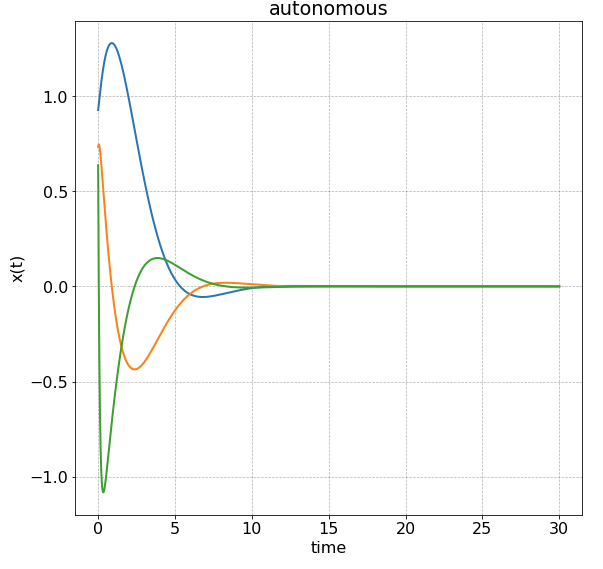
\includegraphics[width=\linewidth]{Autonomous.png}
%\caption{Autonomous ODE ($u = 0$)}
%\endminipage\hfill
%\minipage{0.32\textwidth}
%  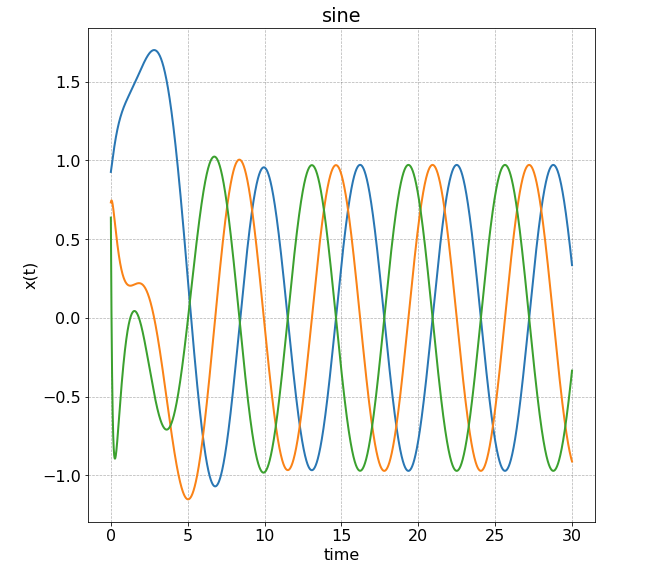
\includegraphics[width=\linewidth]{sine.png}
%\caption{reaction to sine wave ($u = sin(t)$)}
%\endminipage\hfill
%\minipage{0.32\textwidth}%
%  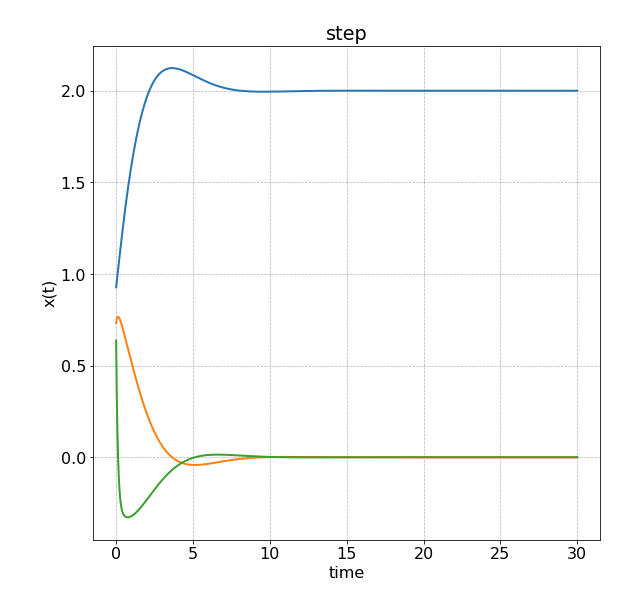
\includegraphics[width=\linewidth]{step.png}
%\caption{Reaction to step function ($u = 1$)}
%\endminipage
%\end{figure}
%
%\end{flushleft}
%\end{frame}


\begin{frame}{Laplace Transform}
% \framesubtitle{O}
\begin{flushleft}

By definition, Laplace transform of a function $f(t)$ is given as:

\begin{equation}
    F(s) = \int_0^\infty f(t) e^{-st}dt
\end{equation}

where $F(s)$ is called an \emph{image} of the function.

\bigskip

The study of Laplace transform is a separate mathematical field with applications in solving ODEs, which we won't cover. However, we will consider transform of one case of interest - transform of a derivative. 

\end{flushleft}
\end{frame}



\begin{frame}{Laplace Transform of a derivative}
% \framesubtitle{O}
\begin{flushleft}

Consider a derivative $\frac{dx}{dt}$ and its transform:

\begin{equation}
    \mathcal{L}\left(\frac{dx}{dt}\right) = \int_0^\infty \frac{dx}{dt} e^{-st}dt
\end{equation}

we will make use of the integration by parts formula:

\begin{block}{Integration by parts}
\begin{equation}
\int v \frac{du}{dt} dt = vu - 
\int \frac{dv}{dt} u dt    
\end{equation}
\end{block}

In our case, $\frac{du}{dt} = \frac{dx}{dt}$, $u = x$, $v = e^{-st}$, $\frac{dv}{dt} = -se^{-st}$:

\begin{equation}
\mathcal{L}\left(\frac{dx}{dt}\right) = \left[x e^{-st} \right]_0^\infty - 
\int_0^\infty -se^{-st} x dt  
\end{equation}

\begin{equation}
\mathcal{L}\left(\frac{dx}{dt}\right) = -x(0) + s\mathcal{L}(x)  
\end{equation}

\end{flushleft}
\end{frame}




\begin{frame}{Derivative operator}
% \framesubtitle{O}
\begin{flushleft}

Thus, assuming that $x(0) = 0$ and denoting $\mathcal{L}\left( x \right) = X(s)$, we can obtain a \emph{derivative operator}:

\begin{equation}
\label{eq:NoIC_laplace}
\mathcal{L}\left(\frac{dx}{dt}\right) = s \mathcal{L}\left(x\right) = s X(s)
\end{equation}

\bigskip

This form of a derivative operator is very simple to use in practice.

\end{flushleft}
\end{frame}



\begin{frame}{Transfer Function}
% \framesubtitle{O}
\begin{flushleft}

Consider the following ODE, where $u$ is an input (function of time that influences the solution of the ODE):

\begin{equation}
\ddot y + a \dot y + b y = u
\end{equation}

We can rewrite it using the derivative operator:

\begin{equation}
s^2 Y(s) + a s Y(s) + b Y(s) = U(s)
\end{equation}

and then collect $Y(s)$ on the left-hand-side:

\begin{equation}
Y(s) = \frac{1}{s^2 + a s + b} U(s)
\end{equation}

This form is called a \emph{transfer function}.

\end{flushleft}
\end{frame}


\begin{frame}{Transfer Function}
\framesubtitle{Examples}
\begin{flushleft}

\begin{example}
Given ODE: $2 \dddot y + 5\dot y - 40 y = 10 u$

The transfer function for it looks: 
$Y(s)  = \frac{10}{2 s^3 + 5 s - 40} U(s)$
\end{example}


\begin{example}
Given ODE: $2 \dot y - 4 y = u$

The transfer function for it looks: $Y(s) = \frac{1}{2 s - 4} U(s)$
\end{example}


\begin{example}
Given ODE: $3 \dddot y + 4y = u$

The transfer function for it looks: $Y(s) = \frac{1}{2 s^3 + 4} U(s)$
\end{example}

\end{flushleft}
\end{frame}




\begin{frame}{Transfer Functions}
\framesubtitle{Interesting things done easy}
\begin{flushleft}

Consider the following (strange) ODE:

\begin{equation}
2 \ddot y + 3 \dot y + 2 y = 10 \dot u - u
\end{equation}

Using the differential equation:

\begin{equation}
2 s^2 Y(s) + 3s Y(s) + 2Y(s) = 10s U(s) - U(s)
\end{equation}

...which is the same as:

\begin{equation}
(2s^2 + 3s + 2) Y(s) = (10s - 1)U(s)
\end{equation}

The transfer function for it looks: 

\begin{equation}
Y(s) = \frac{10s - 1}{2s^2 + 3s + 2} U(s)
\end{equation}

\end{flushleft}
\end{frame}



\begin{frame}{State-Space to Transfer Function conversion}
% \framesubtitle{O}
\begin{flushleft}

Transfer functions are being used to study the relation between the input and the output of the dynamical system.

\bigskip

Consider standard form state-space dynamical system:

\begin{equation}
\begin{cases}
\dot{\bo{x}} = \bo{A}\bo{x} + \bo{B}\bo{u} \\
     \bo{y}  = \bo{C}\bo{x} + \bo{D}\bo{u}
\end{cases}
\end{equation}

We can rewrite it using the derivative operator:

\begin{equation}
\begin{cases}
s\bo{I}\bo{x} -\bo{A}\bo{x} = \bo{B}\bo{u} \\
\bo{y}  = \bo{C}\bo{x} + \bo{D}\bo{u}
\end{cases}
\end{equation}

and then collect $\bo{x}$ on the left-hand-side: $\bo{x} = (s\bo{I} -\bo{A})^{-1} \bo{B}\bo{u}$

and finally, express $\bo{y}$ out:

\begin{equation}
\bo{y}  = \left( \bo{C}(s\bo{I} -\bo{A})^{-1} \bo{B} + \bo{D} \right) \bo{u}
\end{equation}

\end{flushleft}
\end{frame}





\begin{frame}{System}
	%	\framesubtitle{Interesting things done easy}
	\begin{flushleft}
		
		Consider a linear ODE, and its equivalent representations as a state space equation and as a transfer function:
		
		\begin{align}
			&a_n y^n + ... + a_1 y = b_m u^m + ... + b_1 u
			\\
			&\begin{cases}
				\dot{\bo{x}} = \bo{A}\bo{x} + \bo{B}\bo{u} \\
				\bo{y}  = \bo{C}\bo{x} + \bo{D}\bo{u}
			\end{cases}
		\\
		&Y(s)  = G(s) U(s)
		\end{align}
		
		We can call it a \emph{system} $\mathcal{G}$ to avoid referencing particular representation.
		
	\end{flushleft}
\end{frame}




\begin{frame}{Steady-State gain}
	%	\framesubtitle{Interesting things done easy}
	\begin{flushleft}
		
		If a system  $\mathcal{G}$ is stable and given constant input $u_0$ its output is approaching some constant value $y_0$, we can call this pair a \emph{steady-state solution}. The ratio between $y_0$ and $u_0$ is a \emph{steady-state gain} - how much does the system increase the input signal.
		
		Assume the system  $\mathcal{G}$ represented as a transfer function:
		
		\begin{equation}
			Y(s) = \frac{b_m s^m + ... + b_1}{a_n s^n + ... + a_1} U(s)
		\end{equation}
	
		Then, as any element multiplied by the differential operator $s$ with power higher than 0 is a derivative of $u$ or $y$ and both are 0 at the steady-state solution, the steady-state gain can be found by setting those to zero:
		
		\begin{equation}
			K = \frac{b_1}{a_1}
		\end{equation}		
		
		
		
	\end{flushleft}
\end{frame}



\begin{frame}{Transfer Function and Control (1)}
	% \framesubtitle{O}
	\begin{flushleft}
		
		Let the dynamic system be described as a transfer function:
		
		\begin{equation}
			Y(s) = G(s) U(s)
		\end{equation}
		
		We can try to modify the input based on how the output looks. Since we always do it in a linear way, we can write it as:
		
		\begin{align}
			Y(s) = G(s) (U(s) - H(s) Y(s)) 
		\end{align}
		
		where $H(s) y$ is called \emph{feedback}.
		
		\bigskip
		
		How would the transfer function from $U(s)$ to $Y(s) $ look like? 
		
	\end{flushleft}
\end{frame}


\begin{frame}{Transfer Function and Control (2)}
	% \framesubtitle{O}
	\begin{flushleft}
		
		From $Y(s)  = G(s) (U(s)  - H(s) Y(s) )$ we go:
		
		\begin{equation}
			Y(s)  = G(s)U(s) - G(s)H(s) Y(s) 
		\end{equation}
		\begin{equation}
			Y(s)  + G(s)H(s) Y(s)  = G(s)U(s)
		\end{equation}
		\begin{equation}
			Y(s)  = \frac{G(s)}{1 + G(s)H(s)} U(s)
		\end{equation}
		
		Thus, we found \emph{closed-loop} transfer function:
		
		\begin{equation}
			W(s) = \frac{G(s)}{1 + G(s)H(s)}
		\end{equation}
		
	\end{flushleft}
\end{frame}



\begin{frame}{Read more}

\begin{itemize}
\item \bref{https://www.cds.caltech.edu/~murray/courses/cds101/fa04/caltech/am04_ch6-3nov04.pdf}{Chapter 6 Transfer Functions}

\item \bref{https://youtu.be/RJleGwXorUk}{Control Systems Lectures - Transfer Functions, by Brian Douglas}

\item \bref{https://youtu.be/ZGPtPkTft8g}{The Laplace Transform - A Graphical Approach, by Brian Douglas}

\end{itemize}

\end{frame}



\myqrframe

\end{document}
